\subsection{Stazionarietà}
In questo sottocapitolo verrà spiegato il concetto di stazionarietà di una serie
temporale e come poter capire se la serie interessata sia stazionaria.
 
\paragraph{Stazionarietà di una serie temporale}
Per essere stazionaria una serie temporale deve soddisfare
una lista di requisiti:
\begin{enumerate}
    
    \item \textbf{Media costante nel tempo}: La media della serie non deve essere 
    una funzione del tempo. Il grafico rosso, in figura~\ref{fig:nons_mean}, non è stazionario 
    perché la media aumenta nel tempo~\cite{sa:stationary}.

    \begin{figure}[H]
        \centering
        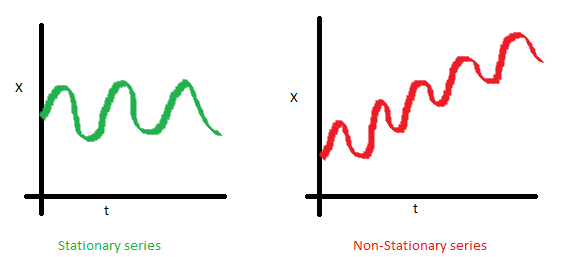
\includegraphics[width=0.65\linewidth,keepaspectratio]{nonstationary_mean.png}
        \caption{Media non costante nel tempo.}
        \label{fig:nons_mean}
    \end{figure}


    \item \textbf{Varianza costante nel tempo}: La varianza della serie non deve 
    essere funzione del tempo. Questa proprietà è nota come omoschedasticità. 
    Nel grafico rosso, in figura~\ref{fig:nons_var}, 
    si noti la variazione della varianza dei dati nel tempo~\cite{sa:stationary}.

    \begin{figure}[H]
        \centering
        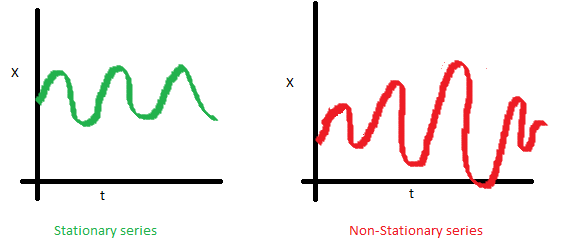
\includegraphics[width=0.65\linewidth,keepaspectratio]{nonstationary_variance.png}
        \caption{Varianza non costante nel tempo.}
        \label{fig:nons_var}
    \end{figure}

    \item \textbf{Covarianza costante nel tempo}: Infine, la covarianza del 
    termine $i$ e del termine $(i + m)$ non deve essere funzione del tempo. 
    Nel grafico, in figura~\ref{fig:nons_cov}, si può notare che lo spread 
    diventa più vicino all'aumentare del tempo. Pertanto, 
    la covarianza non è costante nel tempo per la ``serie rossa''~\cite{sa:stationary}.

    \begin{figure}[H]
        \centering
        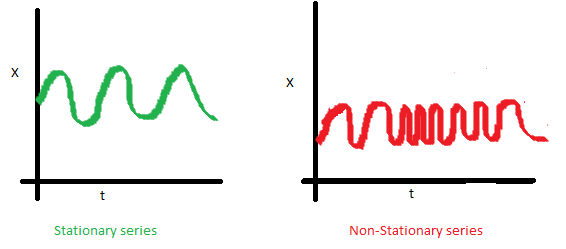
\includegraphics[width=0.65\linewidth,keepaspectratio]{nonstationary_cov.png}
        \caption{Covarianza non costante nel tempo.}
        \label{fig:nons_cov}
    \end{figure}

    Per capire meglio il concetto di covarianza costante nel tempo 
    consideriamo una sequenza di variabili casuali, esse si definiscono
    con stazionarietà debole o stazionarietà della covarianza se:

    \begin{itemize}
        \setlength\itemsep{-0.6em}
        \item Tutti i termini della sequenza hanno la stessa media.
        \item La covarianza tra due termini qualsiasi della sequenza 
        dipende solo dalla posizione relativa dei due termini e non dalla 
        loro posizione assoluta.
    \end{itemize}

    Per posizione relativa di due termini si intende la distanza che 
    li separa l'uno dall'altro nella sequenza mentre per posizione assoluta, 
    si riferisce al punto in cui si trovano nella sequenza~\cite{sl:cov_stat}.

    \begin{figure}[H]
        \centering
        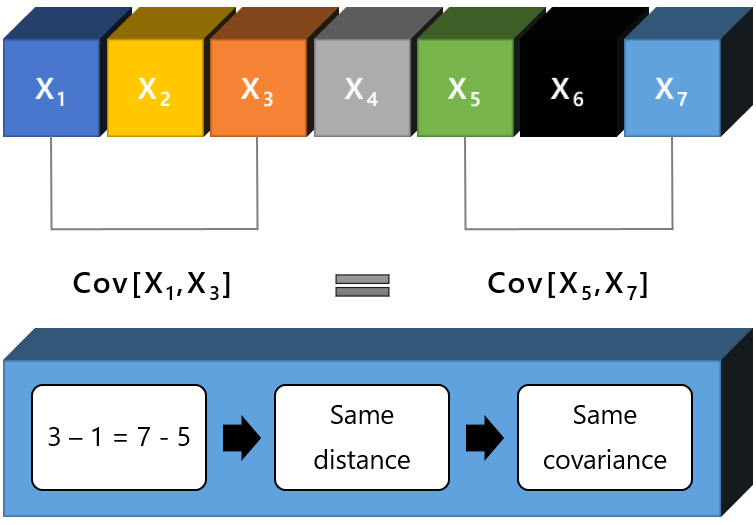
\includegraphics[width=0.4\linewidth,keepaspectratio]{stationary_cov.png}
        \caption{Stazionarietà della covarianza.}
    \end{figure}

\end{enumerate}

\paragraph{L'importanza di una serie stazionaria} 
L'importanza di avere una serie temporale stazionaria deriva dal fatto che 
molti dei teoremi che a livello statistico valgono per le variabili casuali indipendenti
valgono anche per variabili casuali stazionarie~\cite{sa:stationary}.


\subsubsection{Dickey Fuller Test}
Ci sono due modi per verificare la stazionarietà di una serie temporale. 
Il primo consiste nell'osservare i dati. Visualizzando i dati dovrebbe essere 
facile identificare una variazione della media o una variazione dei dati. 
Per una valutazione più accurata esiste il test di Dickey-Fuller~\cite{sa:stationary}.

In statistica, il test di Dickey Fuller verifica l'ipotesi nulla della presenza
di una radice unitaria in un modello autoregressivo di una serie temporale. 
L'ipotesi alternativa è diversa a seconda della versione del test utilizzata, 
ma di solito è la stazionarietà o la trend-stazionarietà (media e varianza costanti nel tempo)~\cite{wiki:dickey_fuller}.

\paragraph{Modello autoregressivo}
Senza scendere troppo nei dettagli matematici diamo solamente la definizione di 
cos'è un modello autoregressivo: 
In statistica, econometria ed elaborazione dei segnali, 
un modello autoregressivo (AR) è una rappresentazione di 
un tipo di processo casuale; come tale, viene utilizzato 
per descrivere alcuni processi variabili nel tempo in natura, 
economia, comportamento, ecc.
Un semplice modello AR di prim'ordine è
\[ y_t = \rho y_{t-1} + u_t \]
dove $y_t$ è la nostra osservazione all'istante di tempo $t$, $\rho$ è un coefficiente
e $u_t$ è l'errore (assunta essere white noise, quindi stazionaria)~\cite{wiki:dickey_fuller}.

In altre parole, se pensiamo alla nostra serie temporale, ogni osservazione ad istante $t$
dipende da un numero arbitrario osservazioni precedenti più un errore.

Se prendiamo come esempio il modello autoregressivo di prim'ordine mostrato sopra allora
esso si dice avere una radice unitaria se il coefficiente $\rho$ è uguale ad $1$.
Se è presente una radice unitaria allora il processo non sarà stazionario e dipenderà da $t$
(per un approfondimento migliore~\cite{wiki:unit_root} e~\cite{wiki:dickey_fuller}).

\paragraph{Utilizzo del test nella pratica}
Per poter utilizzare questo test nella pratica verranno sfruttate le 
funzionalità del modulo \texttt{statsmodels.tsa.stattools} fornite dal 
pacchetto \texttt{statsmodels} precedentemente utilizzato. Più
precisamente la funzione fornita dal modulo è il test di 
``Dickey-Fuller aumentato'' che fornisce un numero negativo, questo più 
è negativo tanto maggiore è il rifiuto dell'ipotesi nulla che esista una unit root (radice unitaria)
ad un certo livello di confidenza~\cite{wiki:aug_dickey_fuller}.

\subparagraph*{Snippet}
\begin{minted}{python3}
    # import del modulo stattools
    import statsmodels.tsa.stattools as sts

    # esecuzione del test
    adf = sts.adfuller(serie)

    # test statistic
    print('T-stat    : {}'.format(adf[0]))

    # p-value
    print('P-value   : {}'.format(adf[1]))

    # numero di osservazioni utilizzate
    print('n-val-used: {}'.format(adf[3]))

    # valori critici
    print('Valori critici:')
    print('\t1%  : {}'.format(adf[4]["1%"]))
    print('\t5%  : {}'.format(adf[4]["5%"]))
    print('\t10% : {}'.format(adf[4]["10%"]))
\end{minted}


\begin{figure}[H]
    \centering
    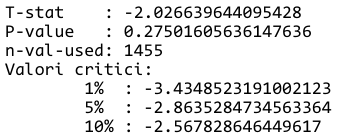
\includegraphics[width=0.4\linewidth,keepaspectratio]{adfuller_test1.png}
    \caption{Output dello snippet sopra indicato (augmented dickey Fuller test).}
    \label{fig:adft_out_ns}
\end{figure}

In questo caso facendo riferimento all'output ottenuto, in figura~\ref{fig:adft_out_ns},
il valore interessato è \texttt{T-stat}, esso è da confrontare con i valori delle variabili
relative alle percentuali di valore critico. Per ogni valore critico controlliamo se
\texttt{T-stat} è maggiore o minore. Nel nostro caso \texttt{T-stat} è maggiore del valore critico
che si riferisce al $10\%$ quindi si ha più del $10\%$ di possibilità che la nostra ipotesi nulla
non sia rifiutata. In altre parole abbiamo più del $10\%$ di possibilità che la nostra
serie temporale non sia stazionaria. Solitamente per considerare una serie temporale 
stazionaria si necessita almeno di $5\%$ quindi un livello di confidenza (che il test rifiuti
l'ipotesi nulla e che quindi vede la nostra serie stazionaria) del $95\%$.
Per semplificarci la vita possiamo direttamente controllare il valore di \texttt{p-value}
(valore compreso tra $0 < \texttt{p-value} < 1$), se esso risulta minore di $0.05$ possiamo considerare
la serie stazionaria.

\paragraph*{Parametri del test}
Per poter applicare correttamente il test di Dickey Fuller su python è necessario
anche impostare i giusti parametri. Se non vengono passati parametri opzionali
il test cerca di trovare la migliore impostazione per la serie. Per poter impostare 
correttamente i parametri del test bisognerebbe andare più nel dettaglio di quest'ultimo 
ma questo esce fuori dallo scopo finale del tirocinio.

\paragraph{Come rendere una serie stazionaria}
Nel caso ci trovassimo difronte ad una serie temporale non stazionaria esistono diverse
tecniche per renderla stazionaria. Una delle tecniche più comuni, e che solitamente funziona per molte
applicazioni, è calcolare la prima differenza (differenza di prim'ordine). Se consideriamo
come $Y$ una serie temporale e con $\hat{Y}$ la medesima dopo aver calcolato la prima 
differenza ogni osservazione di essa sarà definita come
\[ \hat{y}_t = y_{t+1} - y_t \]
dove $\hat{y}_t$ è un'osservazione di $\hat{Y}$ ed $y_{t}$ un'osservazione di $Y$, ad un istante
di tempo $t$.
